\section{Implementation}

Intro: this section is for the technical documentation of the data preprocessing, classifier implementation, explanation generation and validation. 


\subsection{Dataset Selection}
Few datasets with offensive language texts are publicly available. Table \ref{tab:StatsAllDatasets} presents an overview of four available datasets, their sizes and class balances. 
%-------------------------------------------------------
\begin{table}[!ht]
	\centering
	\begin{tabular}{llll}
		\textbf{Corpus} & \textbf{Size} & \textbf{Classes} & \textbf{} \\ \hline
		Davidson\footnote{https://github.com/t-davidson/hate-speech-and-offensive-language} & 25,000 & \begin{tabular}[c]{@{}l@{}} hate speech\\offensive\\neither\end{tabular} & \begin{tabular}[c]{@{}l@{}} 6\%\\77\%\\17\%\end{tabular} \\ \hline
		Imperium\footnote{https://www.kaggle.com/c/detecting-insults-in-social-commentary/data} & 3,947 & \begin{tabular}[c]{@{}l@{}} neutral\\insulting\end{tabular} & \begin{tabular}[c]{@{}l@{}} 73\%\\27\%\end{tabular} \\ \hline
		Analytics Vidhya\footnote{https://datahack.analyticsvidhya.com/contest/practice-problem-twitter-sentiment-analysis/} & 31,962 & \begin{tabular}[c]{@{}l@{}} hate speech\\no hate speech\end{tabular} & \begin{tabular}[c]{@{}l@{}} 7\%\\93\%\end{tabular} \\ \hline
		SwissText\footnote{https://www.swisstext.org/workshops/2018/Hackathon.html} & 159,570 & \begin{tabular}[c]{@{}l@{}} toxic\\severe\_toxic\\obscene\\threat\\insult\\hate speech\\neither\end{tabular} & \begin{tabular}[c]{@{}l@{}} 10\%\\1\%\\5\%\\0.3\%\\5\%\\1\%\\72.7\%\end{tabular} \\ \hline        
	\end{tabular}
	\caption{Publicly available datasets for offensive language texts}
	\label{tab:StatsAllDatasets}
\end{table}
%-------------------------------------------------------
While the dataset of SwissText has the most fine-grained labelling of its data points, details on how the labels were assigned (i.e. number of annotators, inter-annotator agreement score, definition of the classes) are not available. The same holds for the datasets of Analytics Vidhya and Imperium.\newline
In contrast, Davidson's datasets comes with a description of how the data points were collected, how the classes are defined, and uses at least three annotators per text. Furthermore, Davidson's dataset contains the most data points labelled as offensive: roughly 20750 Tweets fall into this category, while the Analytics Vidhya dataset contains 2240 hate speech texts, SwissText 1600, and Imperium 1000.\newline
Throughout the literature, different definitions of hate speech and offensive language are given. For using a dataset in a user study with the scenario of a social media administrator, the definition of the label has to be clear. We therefore chose to work with the dataset of Davidson et al., as it offers the most detailed description of its labels and how the labels were obtained.


\subsection{Dataset Construction}
The original dataset was collected by Davidson et al. \cite{davidson2017automated} for their research on defining and differentiating hate speech from offensive language. They constructed a dataset with offensive Tweets and hate speech by conducting a keyword search on Twitter, using keywords registered in the hatebase dictionary\footnote{https://www.hatebase.org}. The timelines of Twitter users identified with the keyword search were scraped, resulting in a dataset of over 8 million Tweets. They selected 25 000 Tweets at random and had at least 3 annotators from Figure Eight\footnote{https://www.figure-eight.com} (formerly Crowd Flower) who labelled each Tweet as containing hate speech, offensive language, or neither. They reached an inter-annotator agreement of 0.92 \cite{davidson2017automated}. The dataset is publicly available on GitHub\footnote{https://github.com/t-davidson/hate-speech-and-offensive-language}.\newline
The biggest class in the dataset are the offensive language Tweets (77\%), while non-offensive Tweets represent 17\%, and hate speech 6\% of the dataset. \newline
For our research, we are only interested in offensive and not offensive Tweets. We therefore excluded Tweets labelled as hate speech for the further construction of our dataset. We produced a balanced dataset by selecting only Tweets with the maximum inter-annotator agreement from each of the two remaining classes, and randomly drew Tweets from the bigger class (offensive Tweets) until the size of the subset was equal to the size of the smaller class (non-offensive Tweets). Table \ref{tab:StatsDataset} presents statistical information about the resulting dataset.
%-------------------------------------------------------
\begin{table}[!ht]
	\centering
	\begin{tabular}{lll}
		\hline
		\textbf{} & \textbf{Not Offensive Class} & \textbf{Offensive Class} \\ \hline
		Size (absolute) & 4,162 & 4,162 \\
		Size (relative) & 50.00\% & 50.00\% \\
		Total words & 58,288 & 61,504 \\
		Unique words & 6,437 & 9,855 \\
		\begin{tabular}[c]{@{}l@{}}Average words\\per Tweet\end{tabular} & 14.00 & 14.78 \\ \hline         
	\end{tabular}
	\caption{Statistical characteristics of the constructed dataset}
	\label{tab:StatsDataset}
\end{table}
%-------------------------------------------------------




\subsection{Dataset Preprocessing}
Tweets exhibit some special characteristics. First, the maximum length of a single Tweet is 140 characters. Twitter doubled the length in November 2017, yet the dataset was collected before this data and therefore contains only Tweets of 140 characters or shorter. Twitter users found creative ways to make use of the 140 characters given, leading to the usage of short URLs instead of original URLs \cite{xiang2012detecting}, intentional reductions of words (e.g. ``nite" instead of ``night") \cite{xiang2012detecting}, abbreviations \cite{gupta2018proposed}, emojis \cite{ghorai2016information} \cite{watanabe2018hate} and smilies \cite{smailovic2013predictive} \cite{hovelmann2017fasttext}.\newline
Furthermore, social media content can be unstructured, with word creations that are non in standard dictionaries, like slang words \cite{gupta2018proposed} \cite{watanabe2018hate}, intentional repetitions \cite{xiang2012detecting} \cite{hemalatha2012preprocessing} \cite{montani2018tuwienkbs} \cite{rother2018ulmfit} (e.g. ``hhheeeey"), contractions of words \cite{smailovic2013predictive} \cite{hemalatha2012preprocessing}, and spelling mistakes. Although those new word formations do not appear in the dictionary, they are ``intuitive and popular in social media" \cite{hu2012text}. \newline
On Twitter, it is custom to mention other users within a Tweet by adding ``@"+username \cite{xiang2012detecting} \cite{montani2018tuwienkbs} \cite{watanabe2018hate} \cite{rother2018ulmfit}, retweeting (i.e. answering to) a Tweet \cite{xiang2012detecting} \cite{hemalatha2012preprocessing}, and summarizing a Tweet's topic with ``\#"+topic \cite{xiang2012detecting} \cite{watanabe2018hate}. \newline
Other problems in text mining are the handling of stop words \cite{xiang2012detecting} \cite{ghorai2016information} \cite{gupta2018proposed}, language detection \cite{xiang2012detecting}, punctuation \cite{ghorai2016information} \cite{hemalatha2012preprocessing} \cite{montani2018tuwienkbs}, negation \cite{watanabe2018hate}, and case folding \cite{ghorai2016information} \cite{gupta2018proposed} \cite{rother2018ulmfit}.\newline
Researchers have developed different strategies for preprocessing Tweets. One possible approach is to simply remove URLs, username, hashtags, emoticons, stop words, or punctuation \cite{xiang2012detecting} \cite{ghorai2016information} \cite{hemalatha2012preprocessing} \cite{montani2018tuwienkbs} \cite{gupta2018proposed} \cite{watanabe2018hate}. A reason to eliminate those tokens can be that they assumably do not hold information relevant to the classification goal \cite{hemalatha2012preprocessing}. Words that only exist for syntactic reasons (this concerns primarily stop words) can be omitted when focussing on sentiment or other semantic characteristics \cite{ghorai2016information}. Mentions of other users are likewise not informative for sentiment analysis and are often removed from the texts \cite{xiang2012detecting} \cite{watanabe2018hate}. Depending on the dataset size, normalising the texts strongly by removing punctuation and emojis, as well as lowercasing the texts, can decrease the vocabulary size \cite{ghorai2016information}. Especially on Twitter with its restricted text size, users tend to use shortened URLs. Short URLs have a concise, but often cryptic form, and redirect to the website with the original, long URL. While website links can encode some information on a topic, this information is lost when using a shortened URL. Removing the shortened URLs without replacement can be a step in preprocessing Tweets \cite{xiang2012detecting}.\newline
Rather than removing tokens, they can also be replaced by a signifier token, e.g. a complete link by ``$<<<$hyperlink$>>>$" \cite{hovelmann2017fasttext}. In Tweets, such signifier tokens are used for mentions of usernames \cite{smailovic2013predictive} \cite{hovelmann2017fasttext} \cite{rother2018ulmfit}, URLs \cite{smailovic2013predictive} \cite{hovelmann2017fasttext} \cite{rother2018ulmfit}, smilies \cite{hovelmann2017fasttext} or negations \cite{smailovic2013predictive}. Using signifier tokens eliminates some information, i.e. which user was mentioned or which website was linked, but retains the information that a mention or link exists. Tokens can also be grouped by using signifier tokens, i.e. tokens with similar content are summarised with a single token. \cite{hovelmann2017fasttext} uses this technique to group smilies with similar sentiment and Twitter usernames related to the same company.\newline 
Case folding is often addressed by converting Tweets to lower case \cite{ghorai2016information} \cite{hovelmann2017fasttext} \cite{gupta2018proposed}.\medskip\newline
The following preprocessing steps are taken in chronological order:
\begin{enumerate}
	\item Conversion of all texts to lower cases
	\item Replacement of URLs by a dummy URL (``URL")
	\item Replacement of referenced user names and handles by a dummy handle (``USERNAME")
	\item This dataset encodes emojis in unicode decimal codes, e.g. ``\&\#128512;" for a grinning face. In order to keep the information contained in emojis, each emoji is replaced by its textual description (upper cased and without whitespaces to ensure unity for tokenizing)\footnote{https://www.quackit.com/character\_sets/emoji/}.
	\item Resolving contractions such as ``we're" or ``don't" by replacing contractions with their long version\footnote{https://en.wikipedia.org/wiki/Wikipedia:List\_of\_English\_contractions}.
	\item This dataset uses a few signifiers such as ``english translation" to mark a Tweet that has been translated to English, or ``rt" to mark a Retweet (i.e. a response to a previous Tweet). Since those information have been added retrospectively, we discard them here and delete the signifiers from the texts.
	\item Replacement of all characters that are non-alphabetic and not a hashtag by a whitespace
	\item Replacement of more than one subsequent whitespace by a single whitespace
	\item Tokenization on whitespaces
\end{enumerate}
After training the classifiers, the URL and username tokens are replaced by a more readable version (``http://website.com/website" and ``@username", respectively) to make it easier for participants of the user study to envision themselves in the scenario of a social media administrator reading real-world Tweets. Replacing the tokens by their original URLs and usernames would give the participants more information than the classifiers had; we therefore chose to use a dummy URL and username.\medskip\newline

Following the preprocessing steps, the following Tweet is processed from its original form:
\medskip \hrule \medskip
\begin{verbatim}
	"@WBUR: A smuggler explains how he helped fighters along the \end{verbatim}\begin{verbatim}"Jihadi Highway": http://t.co/UX4anxeAwd"
\end{verbatim}
\medskip \hrule \medskip
into a cleaned version:
\medskip \hrule \medskip
\begin{verbatim}
@username a smuggler explains how he helped fighters along the \end{verbatim}\begin{verbatim}jihadi highway http://website.com/website
\end{verbatim}
\medskip \hrule \medskip





\subsection{Classifier}
Intro

\paragraph{Good System}
L2X 

\paragraph{Medium System}
Logistic Regression with binary (1 / -1) coefficients

\paragraph{Bad System}
Inverse L2X



\subsection{Explanations}
reference to section \ref{subsubsec:explanation_systems}: explanations for text via highlighting of important features (here: words). 

\paragraph{Good System}
L2X mutual information

\paragraph{Medium System}
randomly choosing k words from the words with positive (offensive) or negative (not offensive) class

\paragraph{Bad System}
Inverse good system



\subsection{Graphical User Interface}
\begin{itemize}
	\item the ``environment": administration tool
	\item visualisation of the decisions
	\item visualisation of the explanations (why changing text colour, why those two colours, why not gradient)
\end{itemize}

\begin{figure} [H]
	\centering
	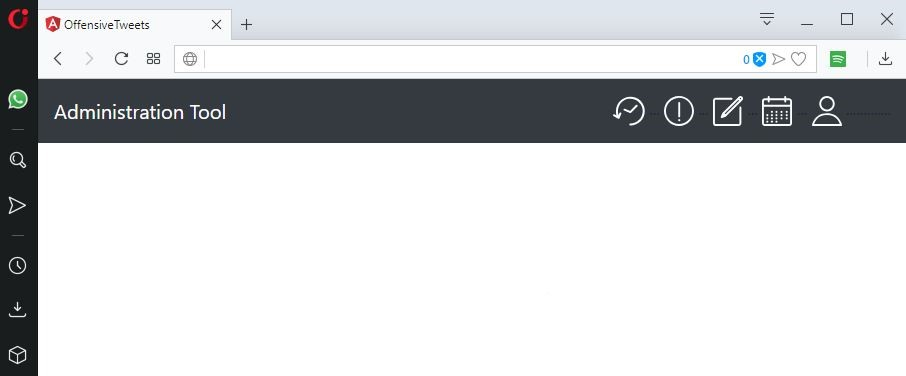
\includegraphics[width=0.8\textwidth]{img/administrationTool.JPG}\\
	\caption{Screenshot of the ``Administration Tool" to support the scenario of a social media administrator}
	\label{fig:admin_tool}
\end{figure}
\begin{figure} [H]
	\centering
	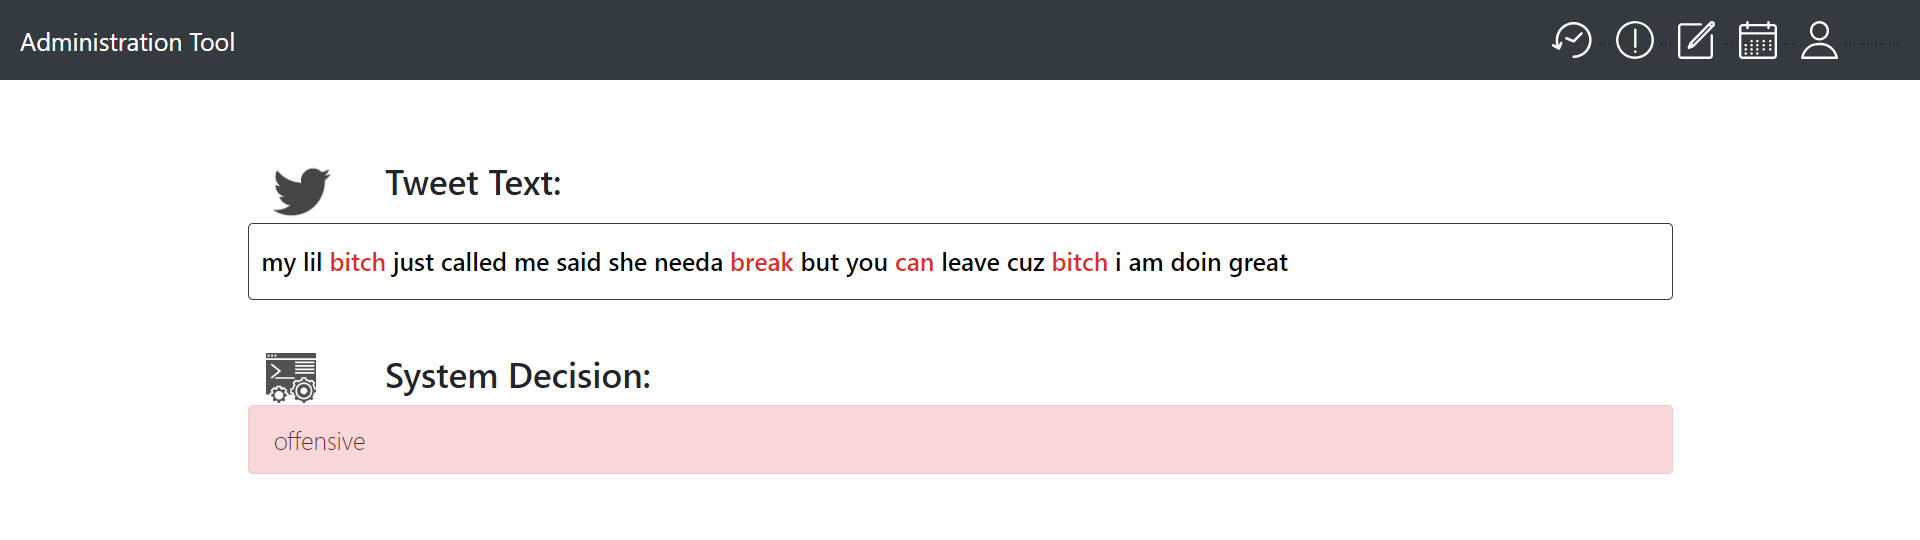
\includegraphics[width=0.8\textwidth]{img/pg_2_12.PNG}\\
	\caption{Screenshot of the ``Administration Tool" showing an offensive Tweet with explanation for its decision}
	\label{fig:admin_tool_offensive}
\end{figure}
\begin{figure} [H]
	\centering
	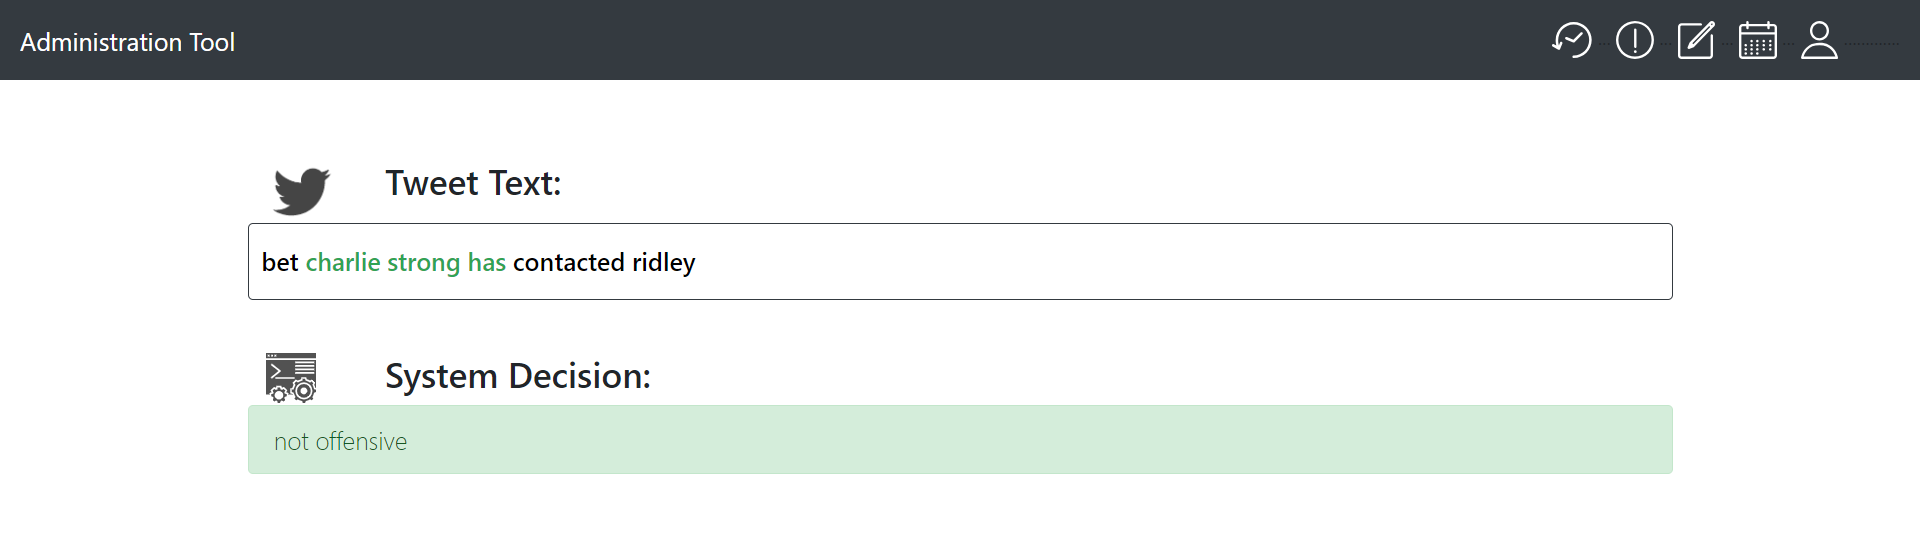
\includegraphics[width=0.8\textwidth]{img/pg_2_0.PNG}\\
	\caption{Screenshot of the ``Administration Tool" showing a non-offensive Tweet with explanation for its decision}
	\label{fig:admin_tool_not_offensive}
\end{figure}



\subsection{Subset Sampling}
For evaluating the different system-explanation conditions, users have to experience the system. However, it is not feasible to present them with the complete testeset, since it has a size of 1665 Tweets. Consequently, a subset of Tweets needs to be drawn from the testset, with a size that a human observer can understand and process within the time frame of a user study.\newline
We furthermore aim to find 10 suitable subsets and assign participants randomly to one of the subsets, in order to reduce possible side effects from biases specific to single Tweets.\newline
There are several requirements for the subsamples, originating from the conflict of reducing the sample for a human observer, yet still yielding a good representation of the testset and classifier:\newline
\begin{itemize}
	\item A class balance of the true labels similar to the testset, 
	\item a balance of correctly to incorrectly classified data points similar to the classifier's performance on the complete testset, 
	\item no overlap of Tweets within the set of 10 subsets,
	\item a feature distribution as close to the feature distribution in the complete testset.
\end{itemize}
We set the subsample size to 15 Tweets, which is enough to show accuracies to the first decimal place, yet assumably not too much to process for an observer in a user study.\newline
To create a subset, 15 data points are randomly drawn from the testset. \newline
First, the class balance of the subset is calculated. The difference to the class balance of the whole testset needs to be smaller than 0.1.\newline
Additionally, for each classifier in the user study, the prediction accuracy on the subset is compared to the prediction accuracy on the complete testset. If, for all classifiers, the difference is smaller than 0.1, the next check is performed.\newline
To ensure the uniqueness of the subsets, the randomly drawn Tweets are compared with the content of previously found subsets. The subset is only accepted if none of the contained Tweets appear in any previously found subset.\newline
In the last step, the feature distribution of the subset is tested against the features of the complete testset using the \textit{Kullback-Leibler Divergence} (KLD) metric. As the focus is directed towards the explanations (i.e. the highlighted words within a Tweet), only the explanations are used to examine the feature distribution. First, the feature distribution of the complete testset is calculated by constructing a word vector with tuples of words and their respective word counts. The word counts are divided by the total amount of words in the set, such that the sum of regularised counts equals 1. Next, a copy of the word vector is used to count and regularise the word frequencies in the subset. The result are two comparable vectors, yet the vector of the subset is very likely to contain zero counts for words that appear in the complete set but were never selected as explanation in the subset. Since the KLD uses the logarithm, it is undefined for zero counts. We use Laplace smoothing with k=1 to handle zero counts. For each classifier, the KLD is calculated and summed to a total divergence score for the subset.\newline
We generate a quantity of 100 such subsets and order them by their KLD sum. The 10 subsets with the smallest score are chosen as the final set of subsets.\newline




\subsection{Explanation Evaluation}
\label{subsec:expleval}
experiments to validate whether the explanations we generate are actually ``good" explanations and those generated with the random method are actually ``bad" explanations.

\subsubsection{Evaluation 1: Accuracy on Reduced Texts}

\subsubsection{Evaluation 2: Ability to Reproduce Classifications}



\subsection{Subset Evaluation}
same as previous section, but with the filtered subsets, basically. And on ``perfect" classifier.